%************************************************
\chapter{Second Year Report}\label{ch:2yearreport} 
%************************************************

\section{Introduction}

More than 50 years after their discovery, no model has yet been developed which is fully able to account for the diverse properties of quasars/AGNs. A more detailed knowledge is required in order to understand the role AGN play in galaxy evolution. The key challenge is relating observables such as the profile of emission/absorption lines and the shape of the spectral energy distribution (SED) to underlying physical properties such as the black-hole (BH) mass and accretion rate. In recent years, significant advances have been made using large spectroscopic and multi-wavelength photometric surveys (most notably SDSS). 

\section{Summary of Work Completed}

In my first year report, I described how I had constructed an SED model which is able to reproduce the average optical to near-infrared (NIR) colours of 10,000s of AGNs spanning a broad range in redshift/luminosity. Broadly, my research involves relating the intrinsic spread in SED properties to physical properties of the AGN. In the 1-3$\mu$m region, the SED is believed to be dominated by thermal emission from hot ($\sim$1200K) dust very close to the central engine and possibly at the inner edge of a dusty torus. By fitting my SED model to the UKIDSS-WISE photometric data I can measure the temperature and abundance of this hot dust component and therefore place constraints on the location and covering factor. We have uncovered a number of interesting results, for example an anti-correlation between the AGN luminosity and the temperature of the hot dust (see Figure~\ref{fig:figure1}). 

\begin{figure}
    \centering
    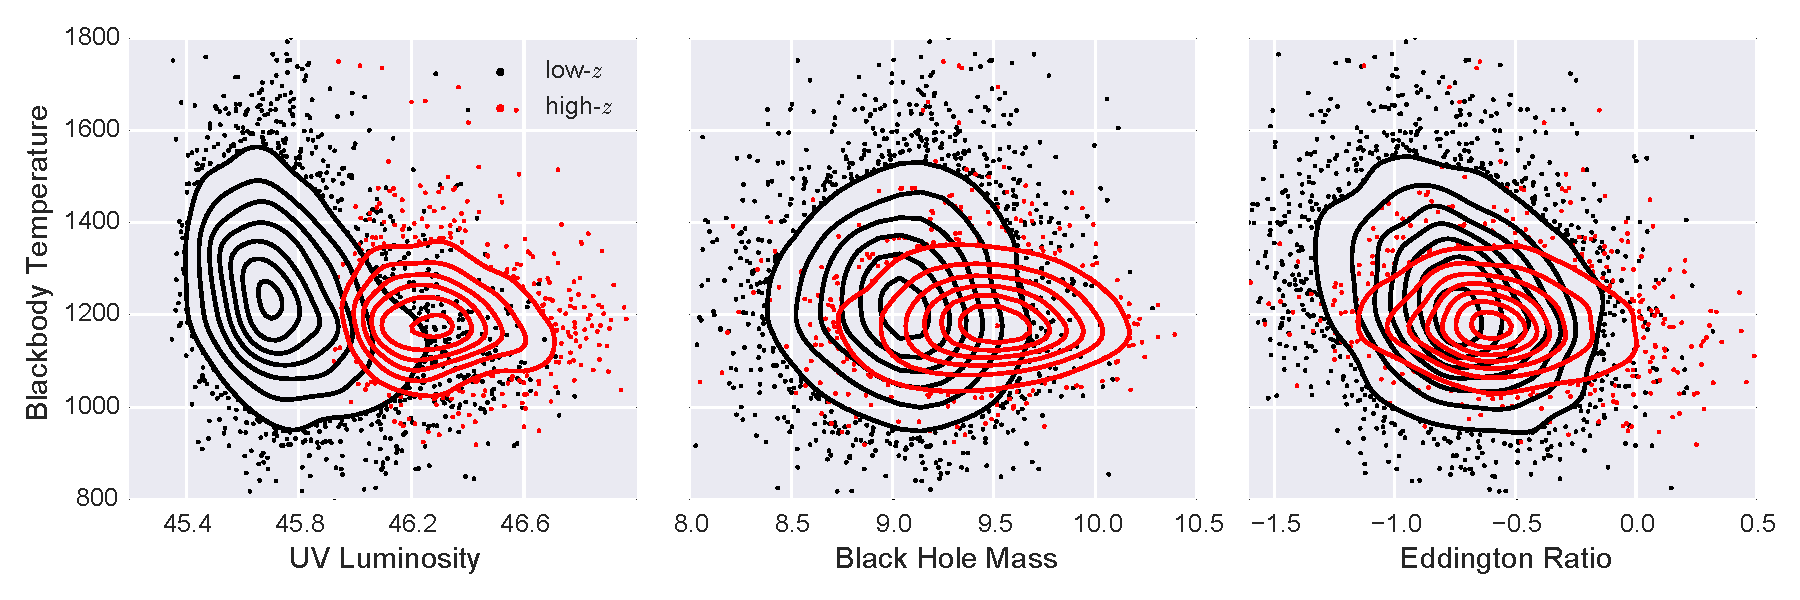
\includegraphics[width=\columnwidth]{figures/chapter05/figure2.pdf}
    \caption{Black-body temperature plotted (from {\it left} to {\it right}) as a function of the ultra-violet luminosity, the black-hole mass and the Eddington ratio.}  
    \label{fig:figure1}
\end{figure}

High-ionization, broad emission lines, such as CIV, are shifted by up to $\sim$3000 km/s blue-ward of the systemic redshift, and the blue-shifted component is thought to arise in an out-flowing wind of highly-ionised material from the accretion disc. A new and much improved scheme from Paul Hewett for determining systemic redshifts allows the blue-shift of the CIV line to be measured very accurately. This has allowed us to show that the blue-shift of the CIV line is correlated with the amount of hot dust emission we measure from the SED. This suggests that either a significant amount of the dust is in the outflow itself or there is some other property of the quasar, such as the orientation with respect to our line-of-sight, which the hot dust and outflows are both dependent on. 

At the end of March we spent four nights using the near-infrared spectrograph on the WHT. We were able to obtain spectra covering H$\alpha$, H$\beta$ and [OIII] for a sample of $\sim$20 quasars with a wide range of outflow and hot dust properties. We have used the broad Balmer lines to measure single-epoch (SE) virial BH mass estimates and have used these estimates to show that BH mass estimates based on the CIV emission line may be overestimated by a factor of $\sim$4 when the CIV line has a significant blue-shifted component (see Figure~\ref{fig:figure2}). We can also use the narrow [OIII] emission line to study outflows on kilo-parsec scales.  

\begin{figure}
    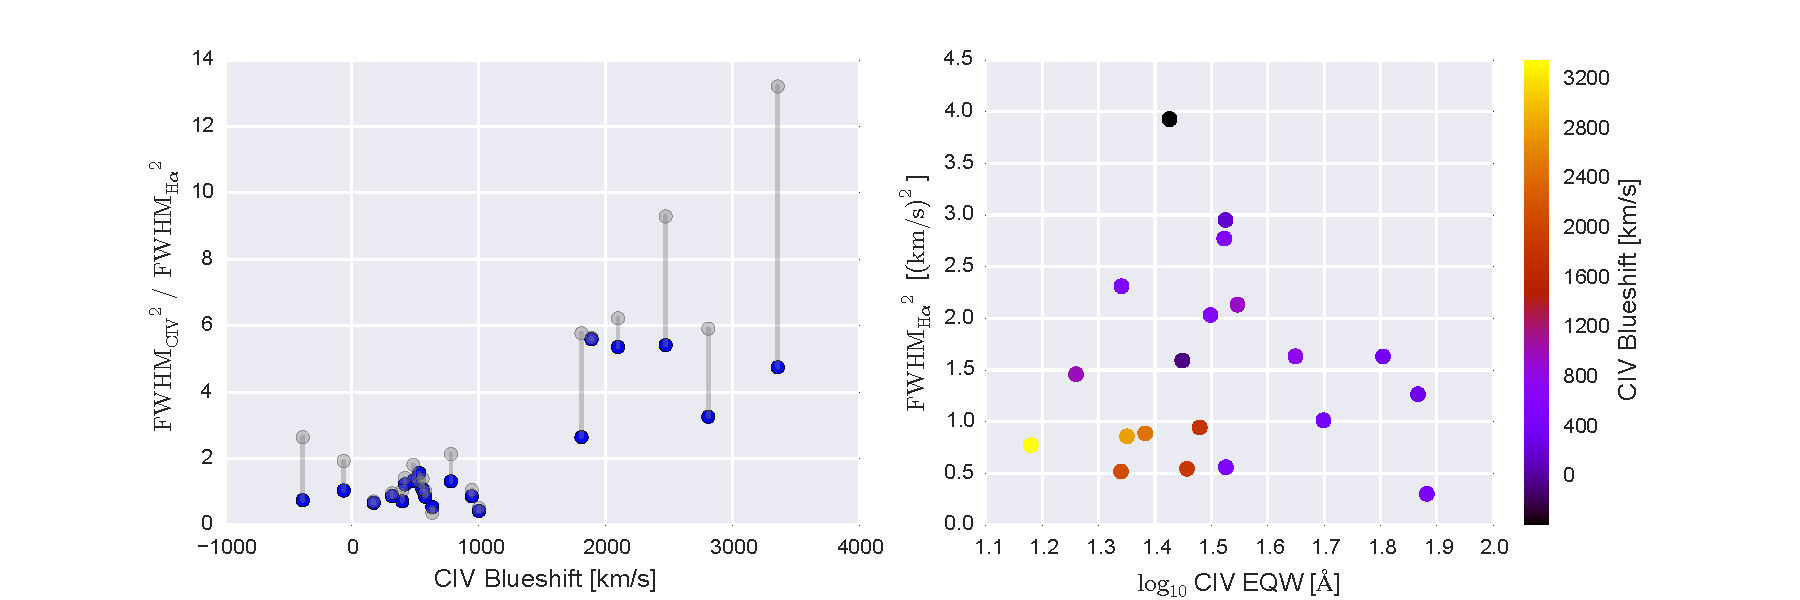
\includegraphics[width=\columnwidth]{figures/chapter05/figure.pdf}
    \caption{{\it Left:} Ratio of ${\rm FWHM_{CIV}}^2$ and ${\rm FWHM_{H\alpha}}^2$  plotted as a function of the CIV blue-shift. {\it Right:} ${\rm FWHM_{H\alpha}}^2$ plotted as function of CIV equivalent width. Note how at high blue-shifts CIV-based BH masses will be overestimated, and how, at low CIV equivalent width, the H$\alpha$-based BH masses are systematically lower for the quasars with blue-shifted CIV.}
    \label{fig:figure2}
\end{figure}

\section{Future Work}

\begin{itemize}
\item Our immediate priority is to publish a paper on how the profile of the CIV line affects SE BH mass estimates in our sample of $\sim$20 luminous quasars. We anticipate that this should be ready to submit by the end of August. 
\item We have obtained fully-reduced Gemini/GNIRS, Palomar/TripleSpec, NTT/SofI, and VLT/X-Shooter near-IR spectra of over 100 luminous quasars from our collaborators. We will use this rich data set to develop our investigation in to outflow properties and BH masses. One goal is to derive a correction to the widely used CIV-based BH mass estimates as a function of the CIV blue-shift. We aim to complete this work by the end of December.  
\item We have been awarded five nights using the near-infrared spectrograph on the NTT at the end of August. We will use this time to ensure our large sample of quasars with near-IR/SDSS optical spectra fully spans the observed range of CIV emission line morphologies and hot dust properties. We also plan to observe the heavily-reddened quasar sample from Banerji et al. 2012-2015, which are believed to be in the process of expelling gas and dust.
\item Although progress in our investigation of the hot dust properties of quasars was slower than anticipated, as I described above the work has produced a number of interesting results. Our challenge now is to develop our interpretation and to decide how to present our results. This will be helped by our now deeper understanding of the biases in the BH masses / Eddington ratios. Much of our hot dust investigation has already been written up, and our plan is to have our first paper completed by the end of February 2016. This work will be built on by, for example, investigating dust-extinction (combining our sample with moderately-reddened quasars from Maddox et al. 2012 and heavily-reddened quasars from Banerji et al. 2012-2015), broad-absorption line quasars, and/or radio properties. We will also investigate the sub-population of quasars for which we don't observe any emission from hot dust. 
\end{itemize}